\chapter{Exploring the Uncanny Valley in Human-Like Robot Recruiters}
\label{chap:6}
Human resource operations are progressively becoming more digital. Many procedures are already automated, and the use of artificial intelligence is also becoming increasingly common. Especially in the recruitment process, a new approach called robot recruiting is being applied. Robot recruitment describes a semi-automatic process in which algorithms and artificial intelligence take over parts of the typical recruiting process, such as assessing and selecting applicants \cite{robot_recruiting}. By analysing vast amounts of data, these algorithms are trained to assist companies in making predictions and decisions on future employees \cite{robot_recruiting_scholar}. This assistance is hoped to shorten the time-consuming process of personnel recruitment and employ a more neutral way of evaluating the applicants \cite{robot_recruiting_scholar}.\\
Many people are already familiar with websites that provide a chat window where one can talk to supposed employees. Often these 'employees' are, in fact, algorithms with which you can communicate, and they can perform a variety of simple tasks \cite{robot_recruiting}. These algorithms are among the best-known applications similar to the intention of robot recruiting. When applying this concept to the recruitment processes, an algorithm takes over the simpler communication and carries out sorting, admission and possibly an exclusion of applicants \cite{robot_recruiting}. However, with the rapid development of information technology, robot recruiters can take on even more complex tasks, such as conducting a job interview \cite{robot_recruiting}. For this task, however, the algorithms need a medium with which to communicate with candidates, and a human-like figure in the shape of an online character or a robot is frequently used for this purpose. One example of this is a Russian start-up which has developed a robot recruitment system called robot Vera, with which companies can conduct telephone interviews with applicants \cite{robot_recruiting}. The robot talks to the applicants self-sufficiently and responds to their questions. During the telephone interview, the robot takes on a female human form \cite{robot_recruiting}.
With the development of a human-like appearance of robot recruiters, the effect of the uncanny valley on them also becomes relevant. If the appearance of a robot recruiter falls into the uncanny valley, it could affect the applicant's acceptance of the recruiter during the interview. This could negatively impact the applicant's behaviour and, therefore, their performance during the application process.
With the help of a survey based on rating possible robot recruiters with varying human-likeness, this thesis explores how applicants' feelings toward different designs of robot recruiters vary.With the survey results, the thesis then tries to determine if very but not perfectly human-like robot recruiters fall into the uncanny valley. The results are also used to make a recommendation for the aspired degree of human-likeness of such entities. 

\section{Stimuli}
For the survey, eight images \ref{fig:image-1} - \ref{fig:image-8} of possible robot recruiters with different human-likeness and a control image of a real human \ref{fig:image-9} were selected. When choosing the entities, special consideration was given to the fact that they either currently exist or may be plausible as a design for a robot recruiter. Among the images are four avatars that are currently in development or use. Figure \ref{fig:image-2} shows the existing Robot Recruiter, Tengai, a physical robot developed to assist recruiters and hiring managers. More information about the company and this robot recruiter can be found on the company's website (https://www.tengai-unbiased.com/tengai-robot/). Image \ref{fig:image-5} shows a design of the robot recruiter Vera, which is developed by a Russian start-up company \cite{vera}. Figure \ref{fig:image-3} shows an avatar of the Microsoft Mesh system, which is currently under development and aims to connect people working remotely in virtual space via Mixed Reality with the help of avatars \cite{microsoft_mesh}. Although this system was not specifically designed for robot recruiting, such a design could easily be imagined. Image \ref{fig:image-4} shows the humanoid robot Sophia, which was developed by the Hong Kong company Hanson Robotics. Sophia became internationally known due to its particularly human appearance and behaviour compared to previous robot variants. The remaining figures \ref{fig:image-1}, \ref{fig:image-6}, \ref{fig:image-7}, \ref{fig:image-8} were chosen to represent a broader range of human-likeness levels and to compare existing appearances to other possibilities. The images are ordered in ascending human-likeness, which was objectively assessed by using the Human Likeness Predictor of the Abot Database (https://www.abotdatabase.info/) and by the addition of the study's evaluation, which is discussed in the following sections. The constant values from figure \ref{fig:image-5} to \ref{fig:image-8} can be explained by the evaluation of the Abot database, which in its current state only gives a rough assessment, and the variations in the human likeness of the picked entities are already very modest.
\begin{table}[b!]
\centering
\resizebox{\linewidth}{!}{%
\begin{tabular}{ll|ll|ll}
\ref{fig:image-1} &Human-Likeness: 47.27 &\ref{fig:image-4} &Human-Likeness: 88.72 &\ref{fig:image-7} &Human-Likeness: 94.55 \\ \hline
\ref{fig:image-2} &Human-Likeness: 65.16 &\ref{fig:image-5} &Human-Likeness: 94.55 &\ref{fig:image-8} &Human-Likeness: 94.55 \\ \hline
\ref{fig:image-3} &Human-Likeness: 84.13 &\ref{fig:image-6} &Human-Likeness: 94.55 &\ref{fig:image-9} &Human-Likeness: 100
\end{tabular}
}
\caption{Rated human-likeness of the figures.}
\label{tab:rated-human-likeness}
\end{table}
\newpage

\begin{figure}[t!]
 \centering
 \subfloat[\cite{icup}\label{fig:image-1}]{%
      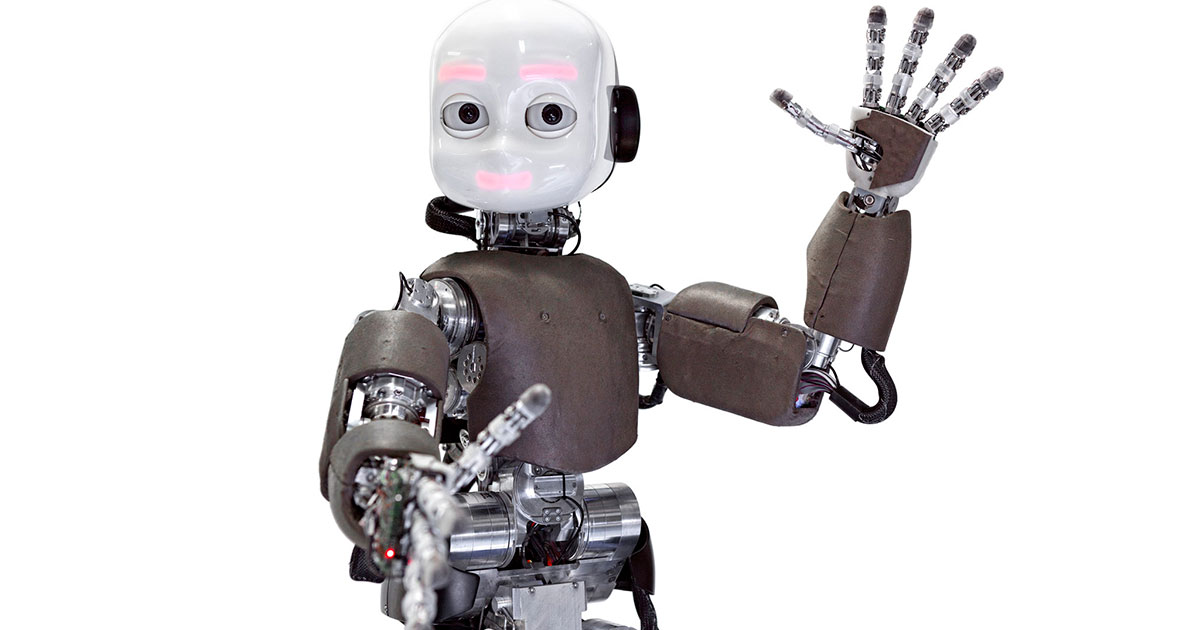
\includegraphics[width=0.26\textwidth]{graphics/study/icup.jpg}}
 \qquad
 \subfloat[\cite{tengai}\label{fig:image-2}]{%
      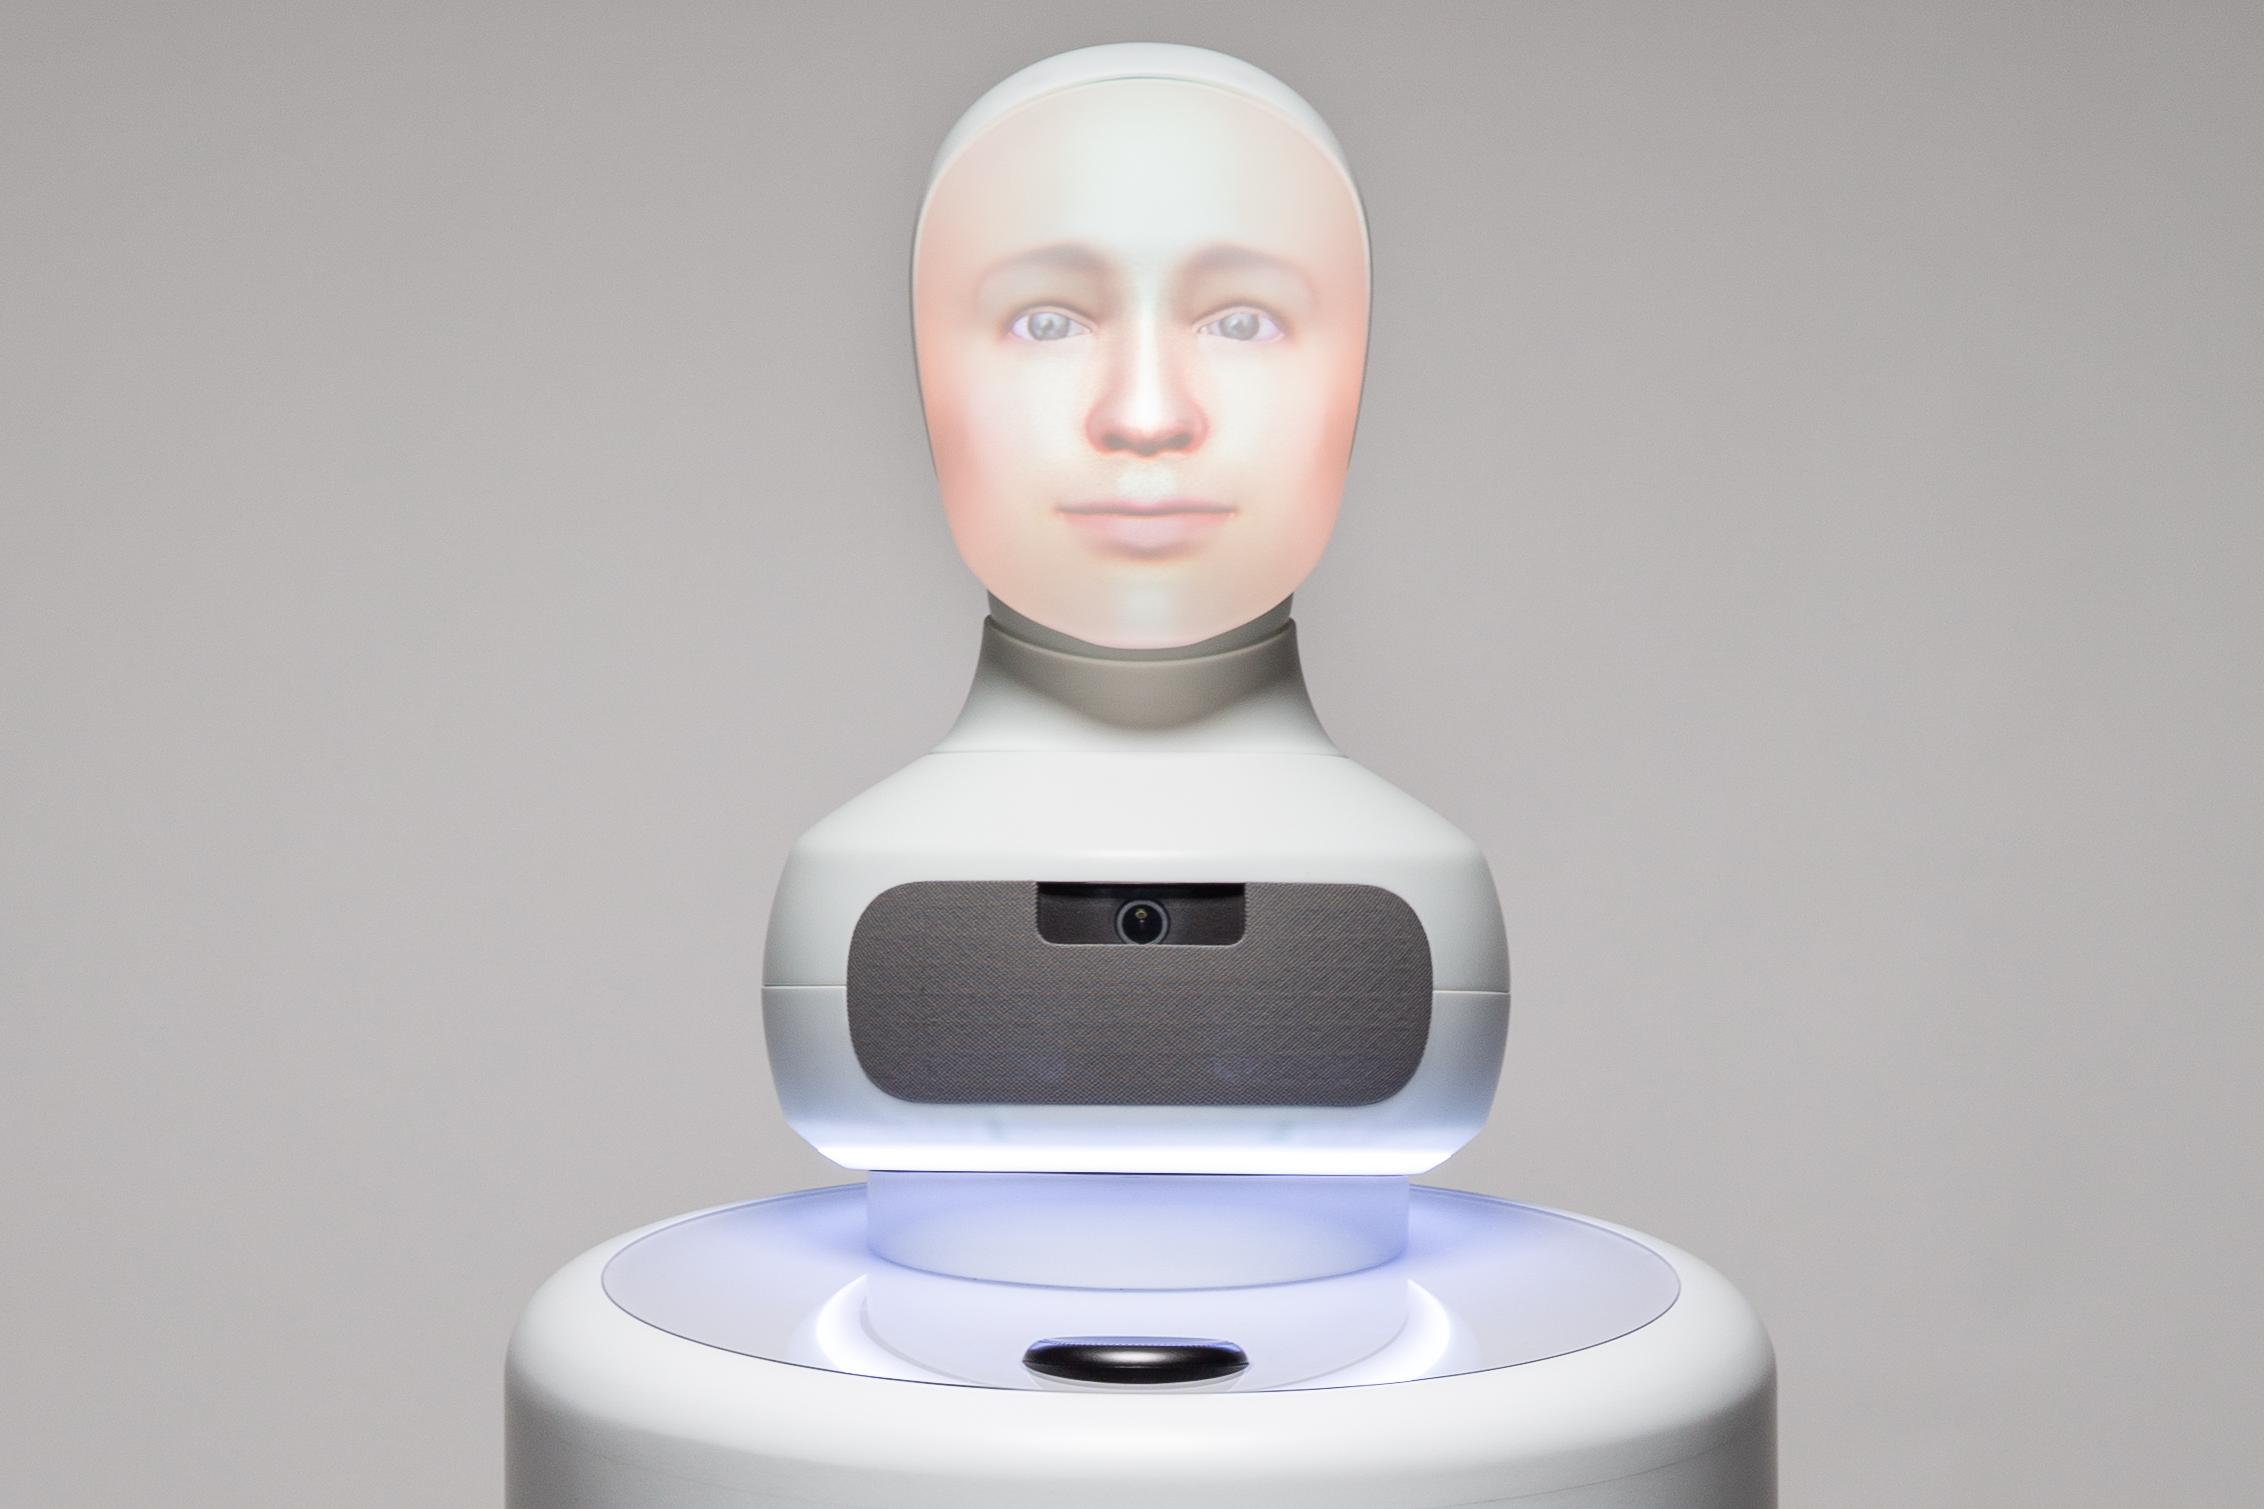
\includegraphics[width=0.26\textwidth]{graphics/study/tengai.jpg}}
 \qquad
 \subfloat[\cite{microsoft_mesh}\label{fig:image-3}]{%
      
\includegraphics[width=0.26\textwidth]{graphics/study/microsoft_mesh.png}}
      
 \centering
  \subfloat[\cite{sophia}\label{fig:image-4}]{%
      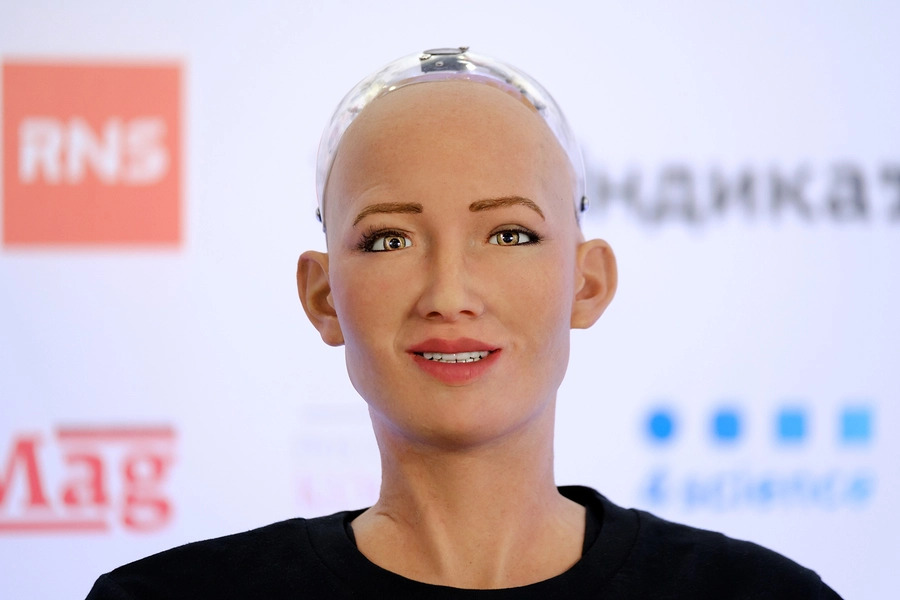
\includegraphics[width=0.26\textwidth]{graphics/study/sophia.jpg}}
 \qquad
 \subfloat[\cite{vera}\label{fig:image-5}]{%
      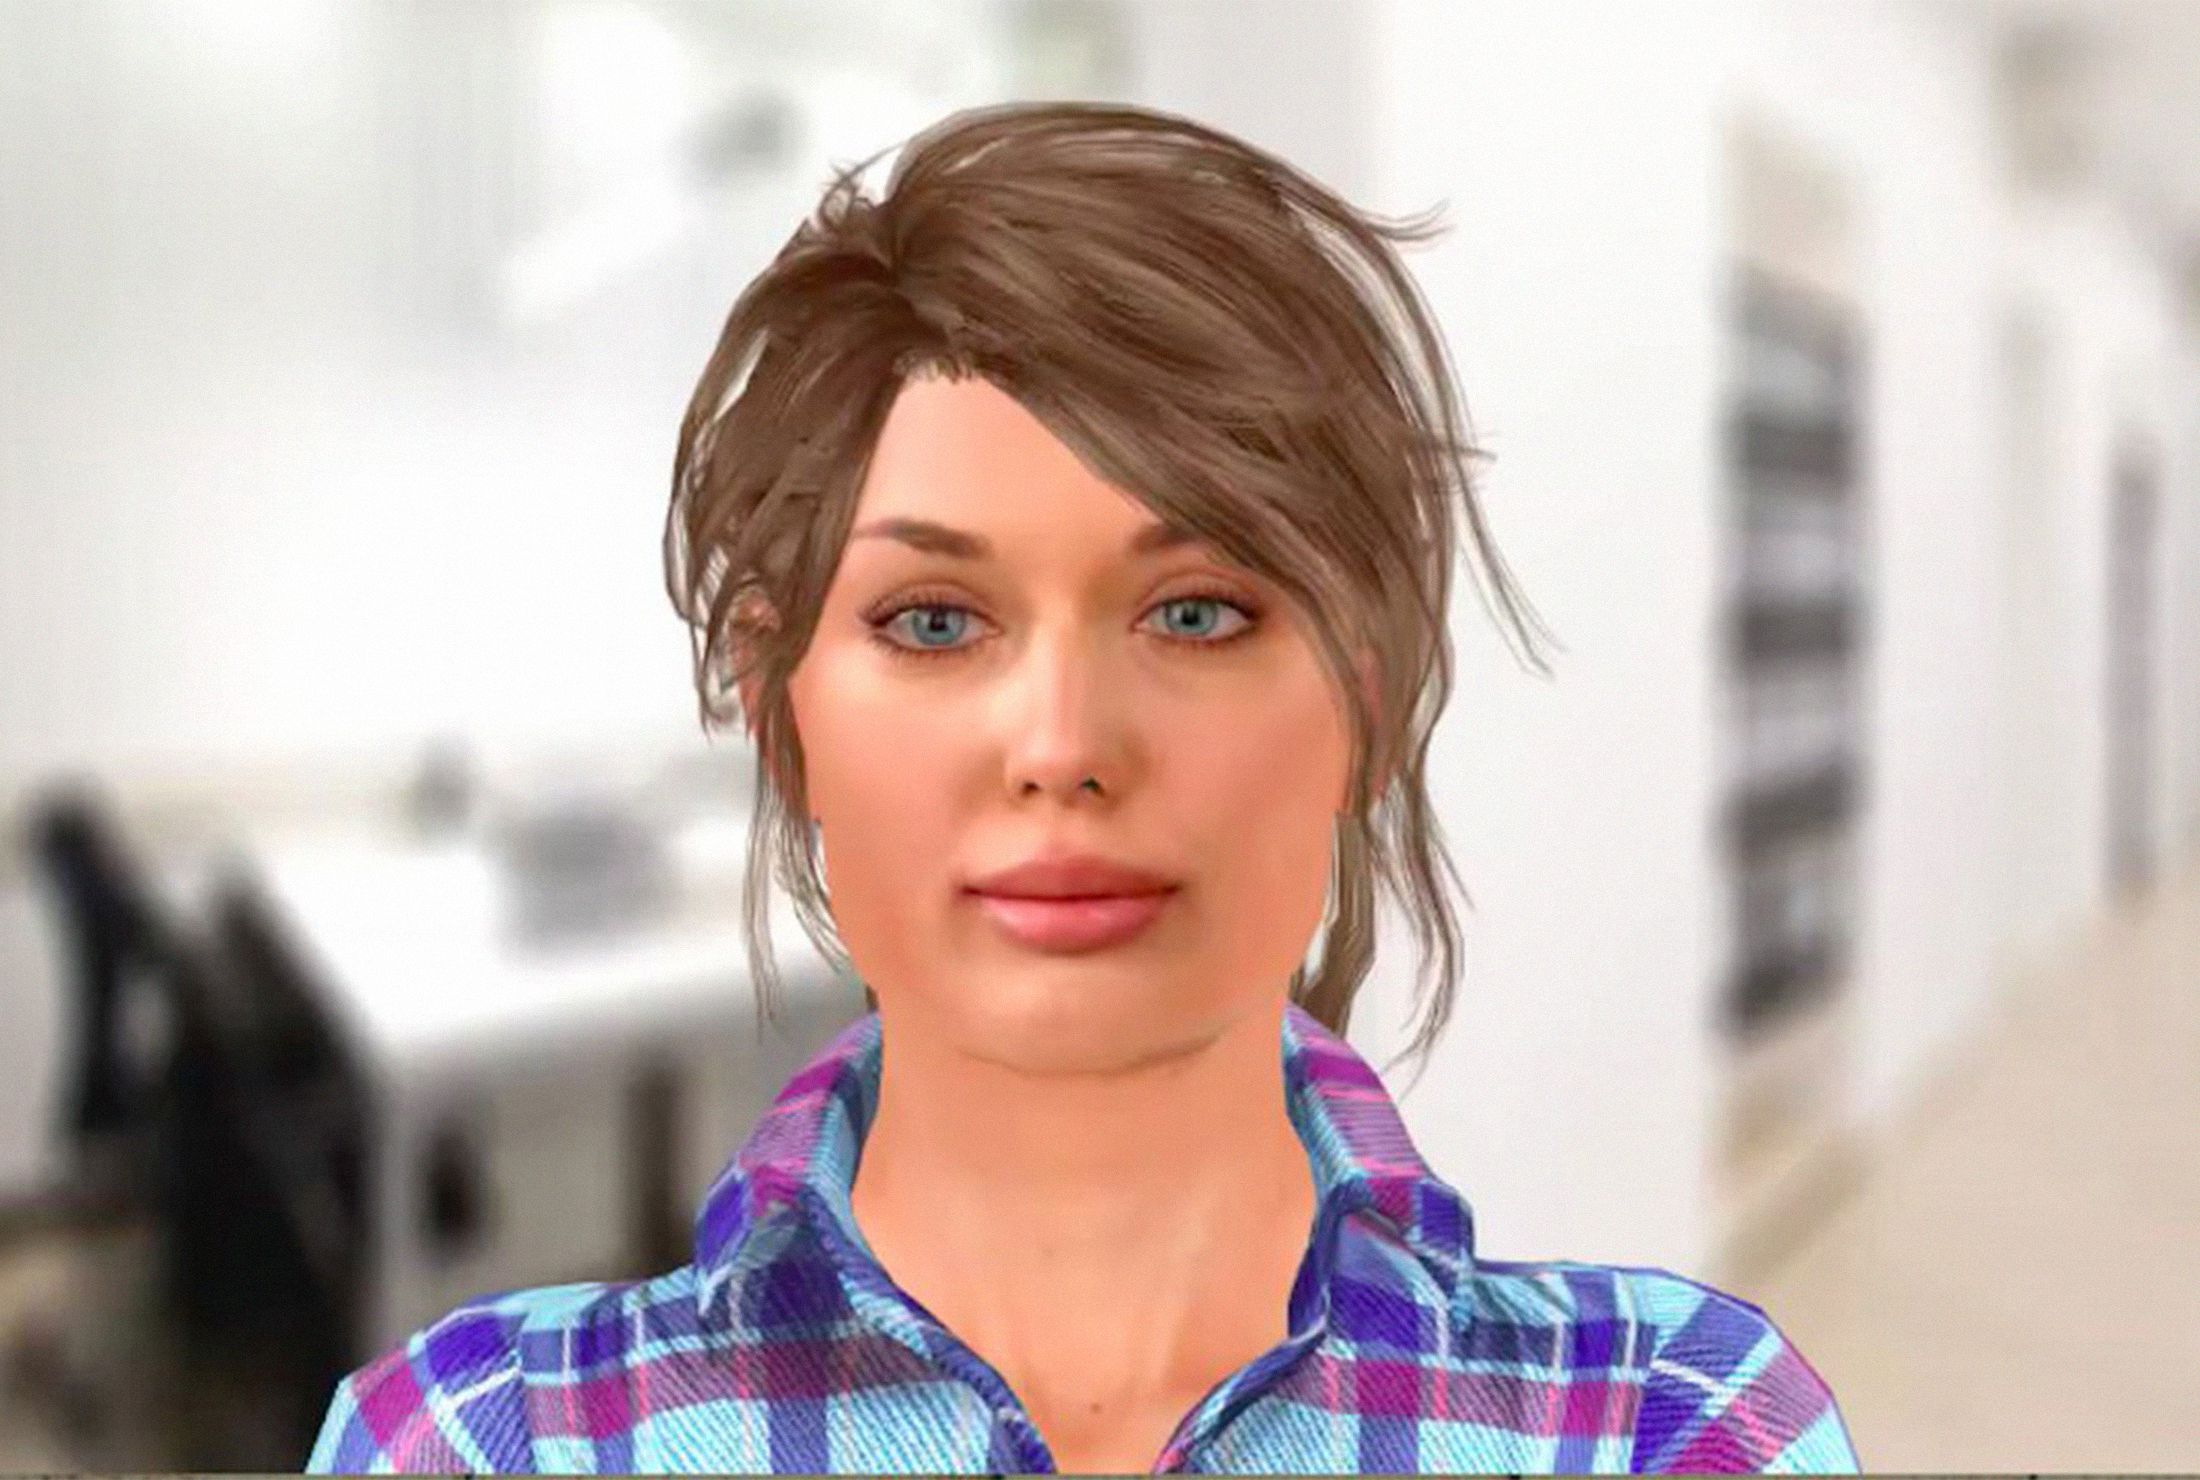
\includegraphics[width=0.26\textwidth]{graphics/study/vera.jpg}}
 \qquad
 \subfloat[\cite{facemaker}\label{fig:image-6}]{%
      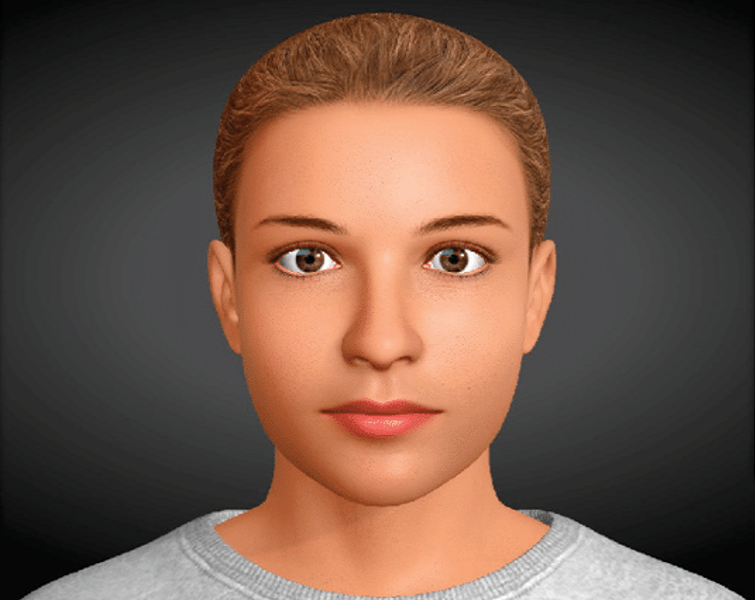
\includegraphics[width=0.26\textwidth]{graphics/study/facemaker.png}}

 \centering
 \subfloat[\cite{knoxfrost}\label{fig:image-7}]{%
      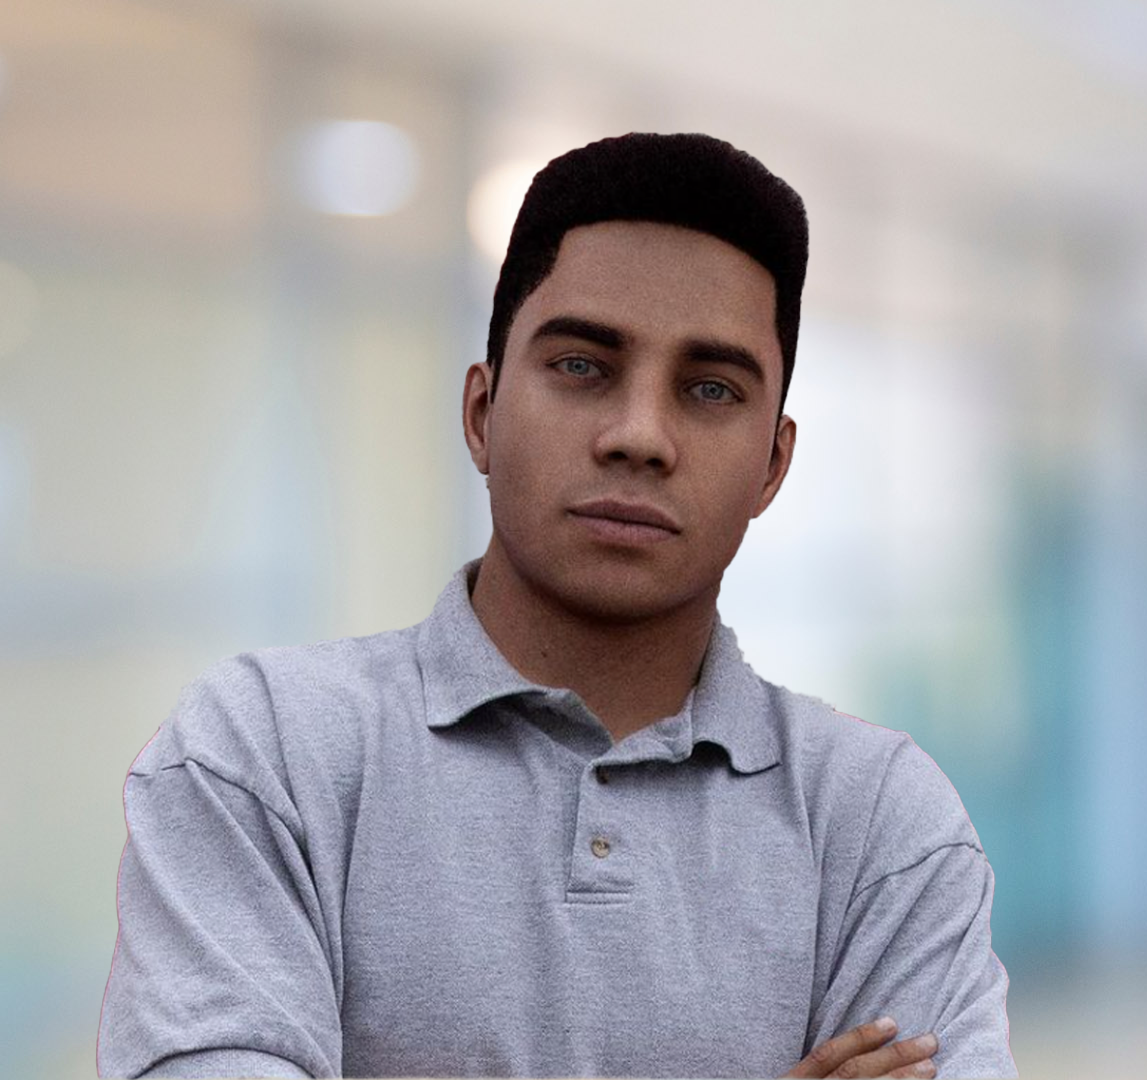
\includegraphics[width=0.26\textwidth]{graphics/study/knoxfrost.png}}
 \qquad
 \subfloat[\cite{emily}\label{fig:image-8}]{%
      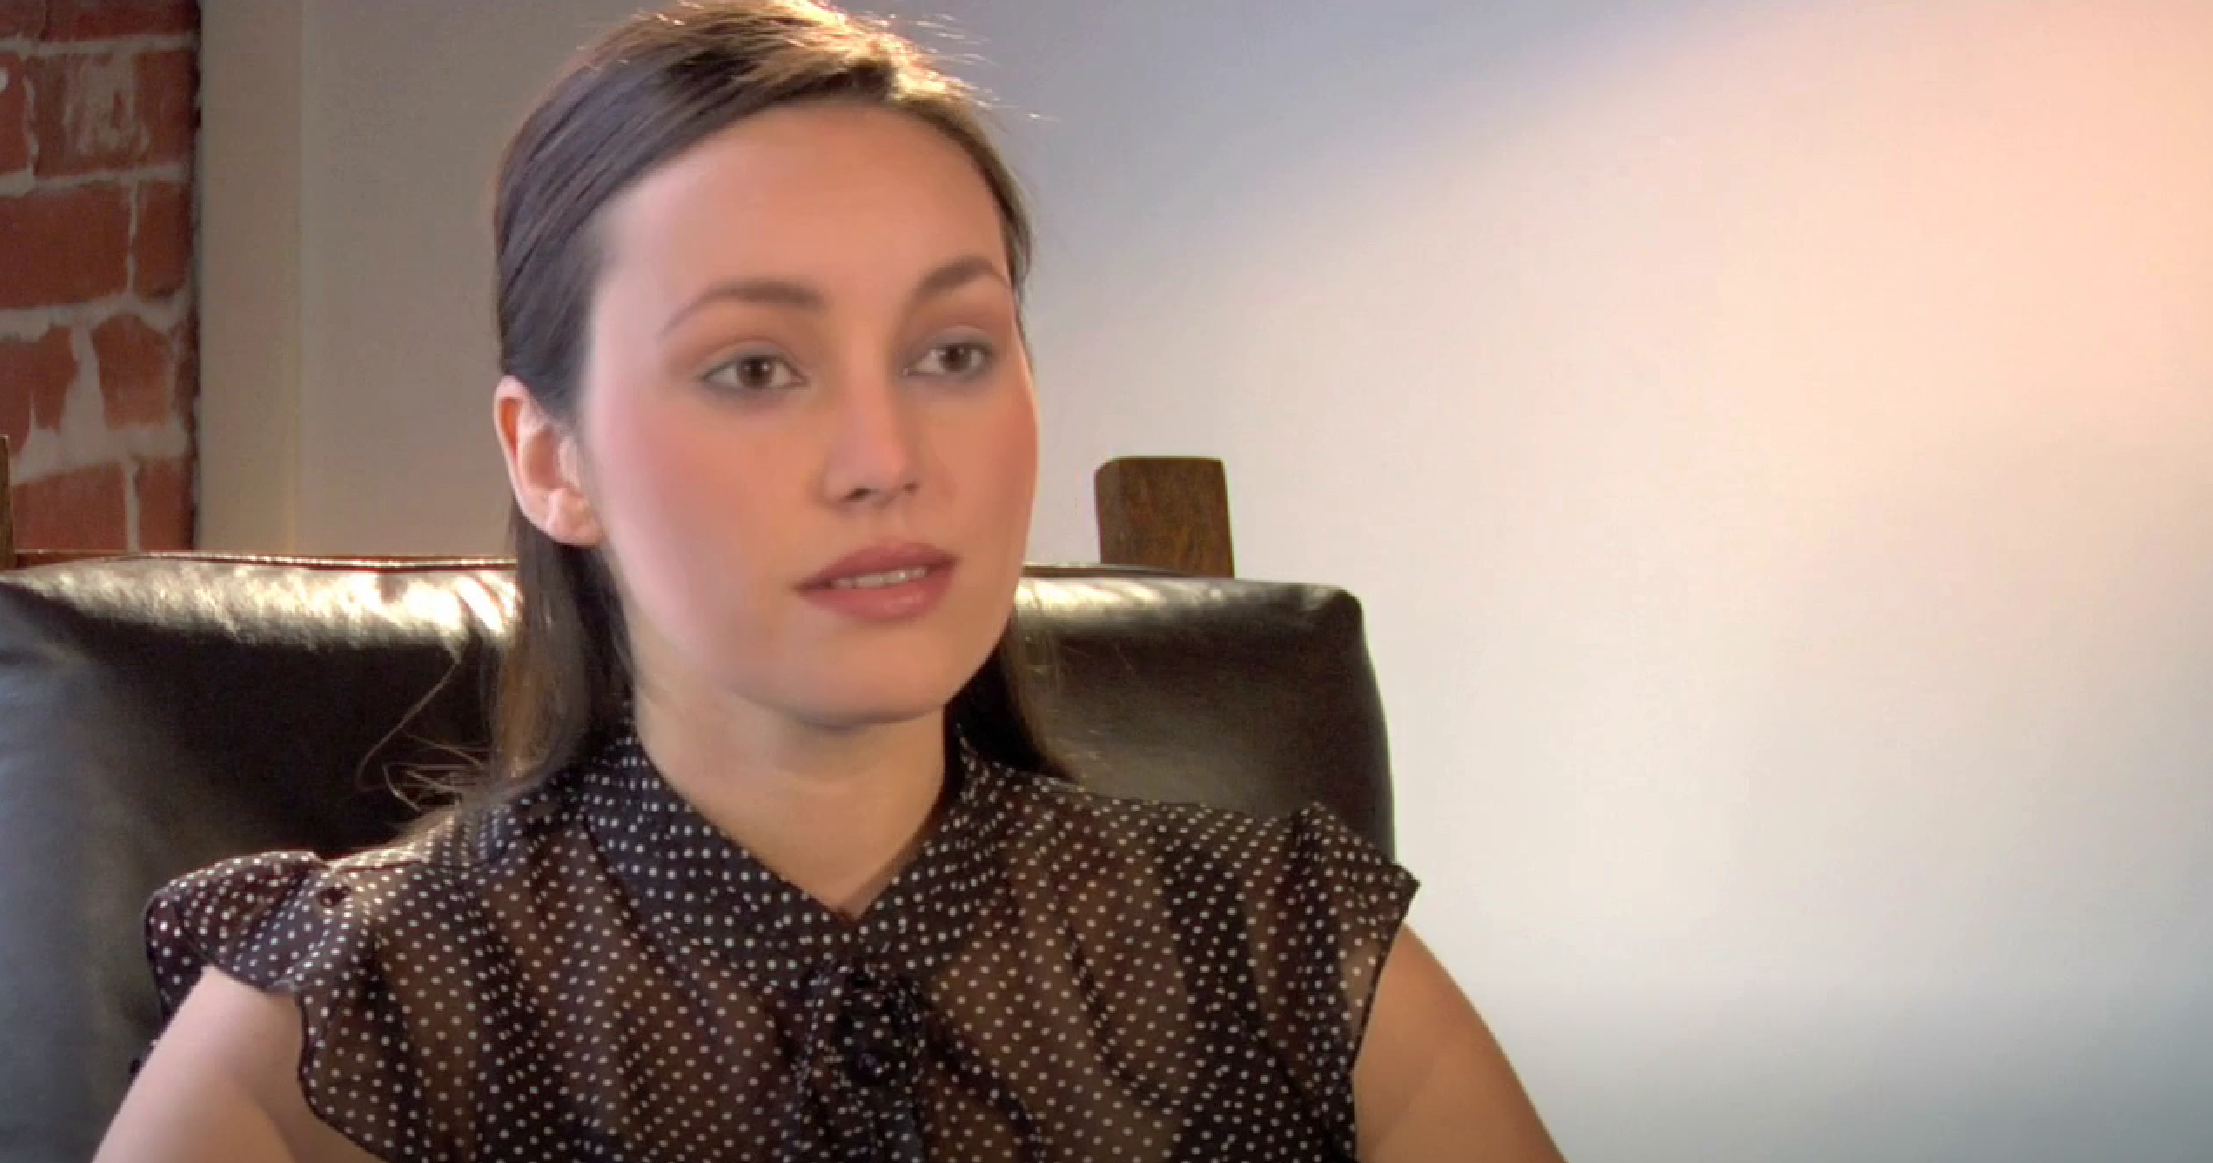
\includegraphics[width=0.26\textwidth]{graphics/study/emily.png}}
 \qquad
 \subfloat[\cite{human}\label{fig:image-9}]{%
      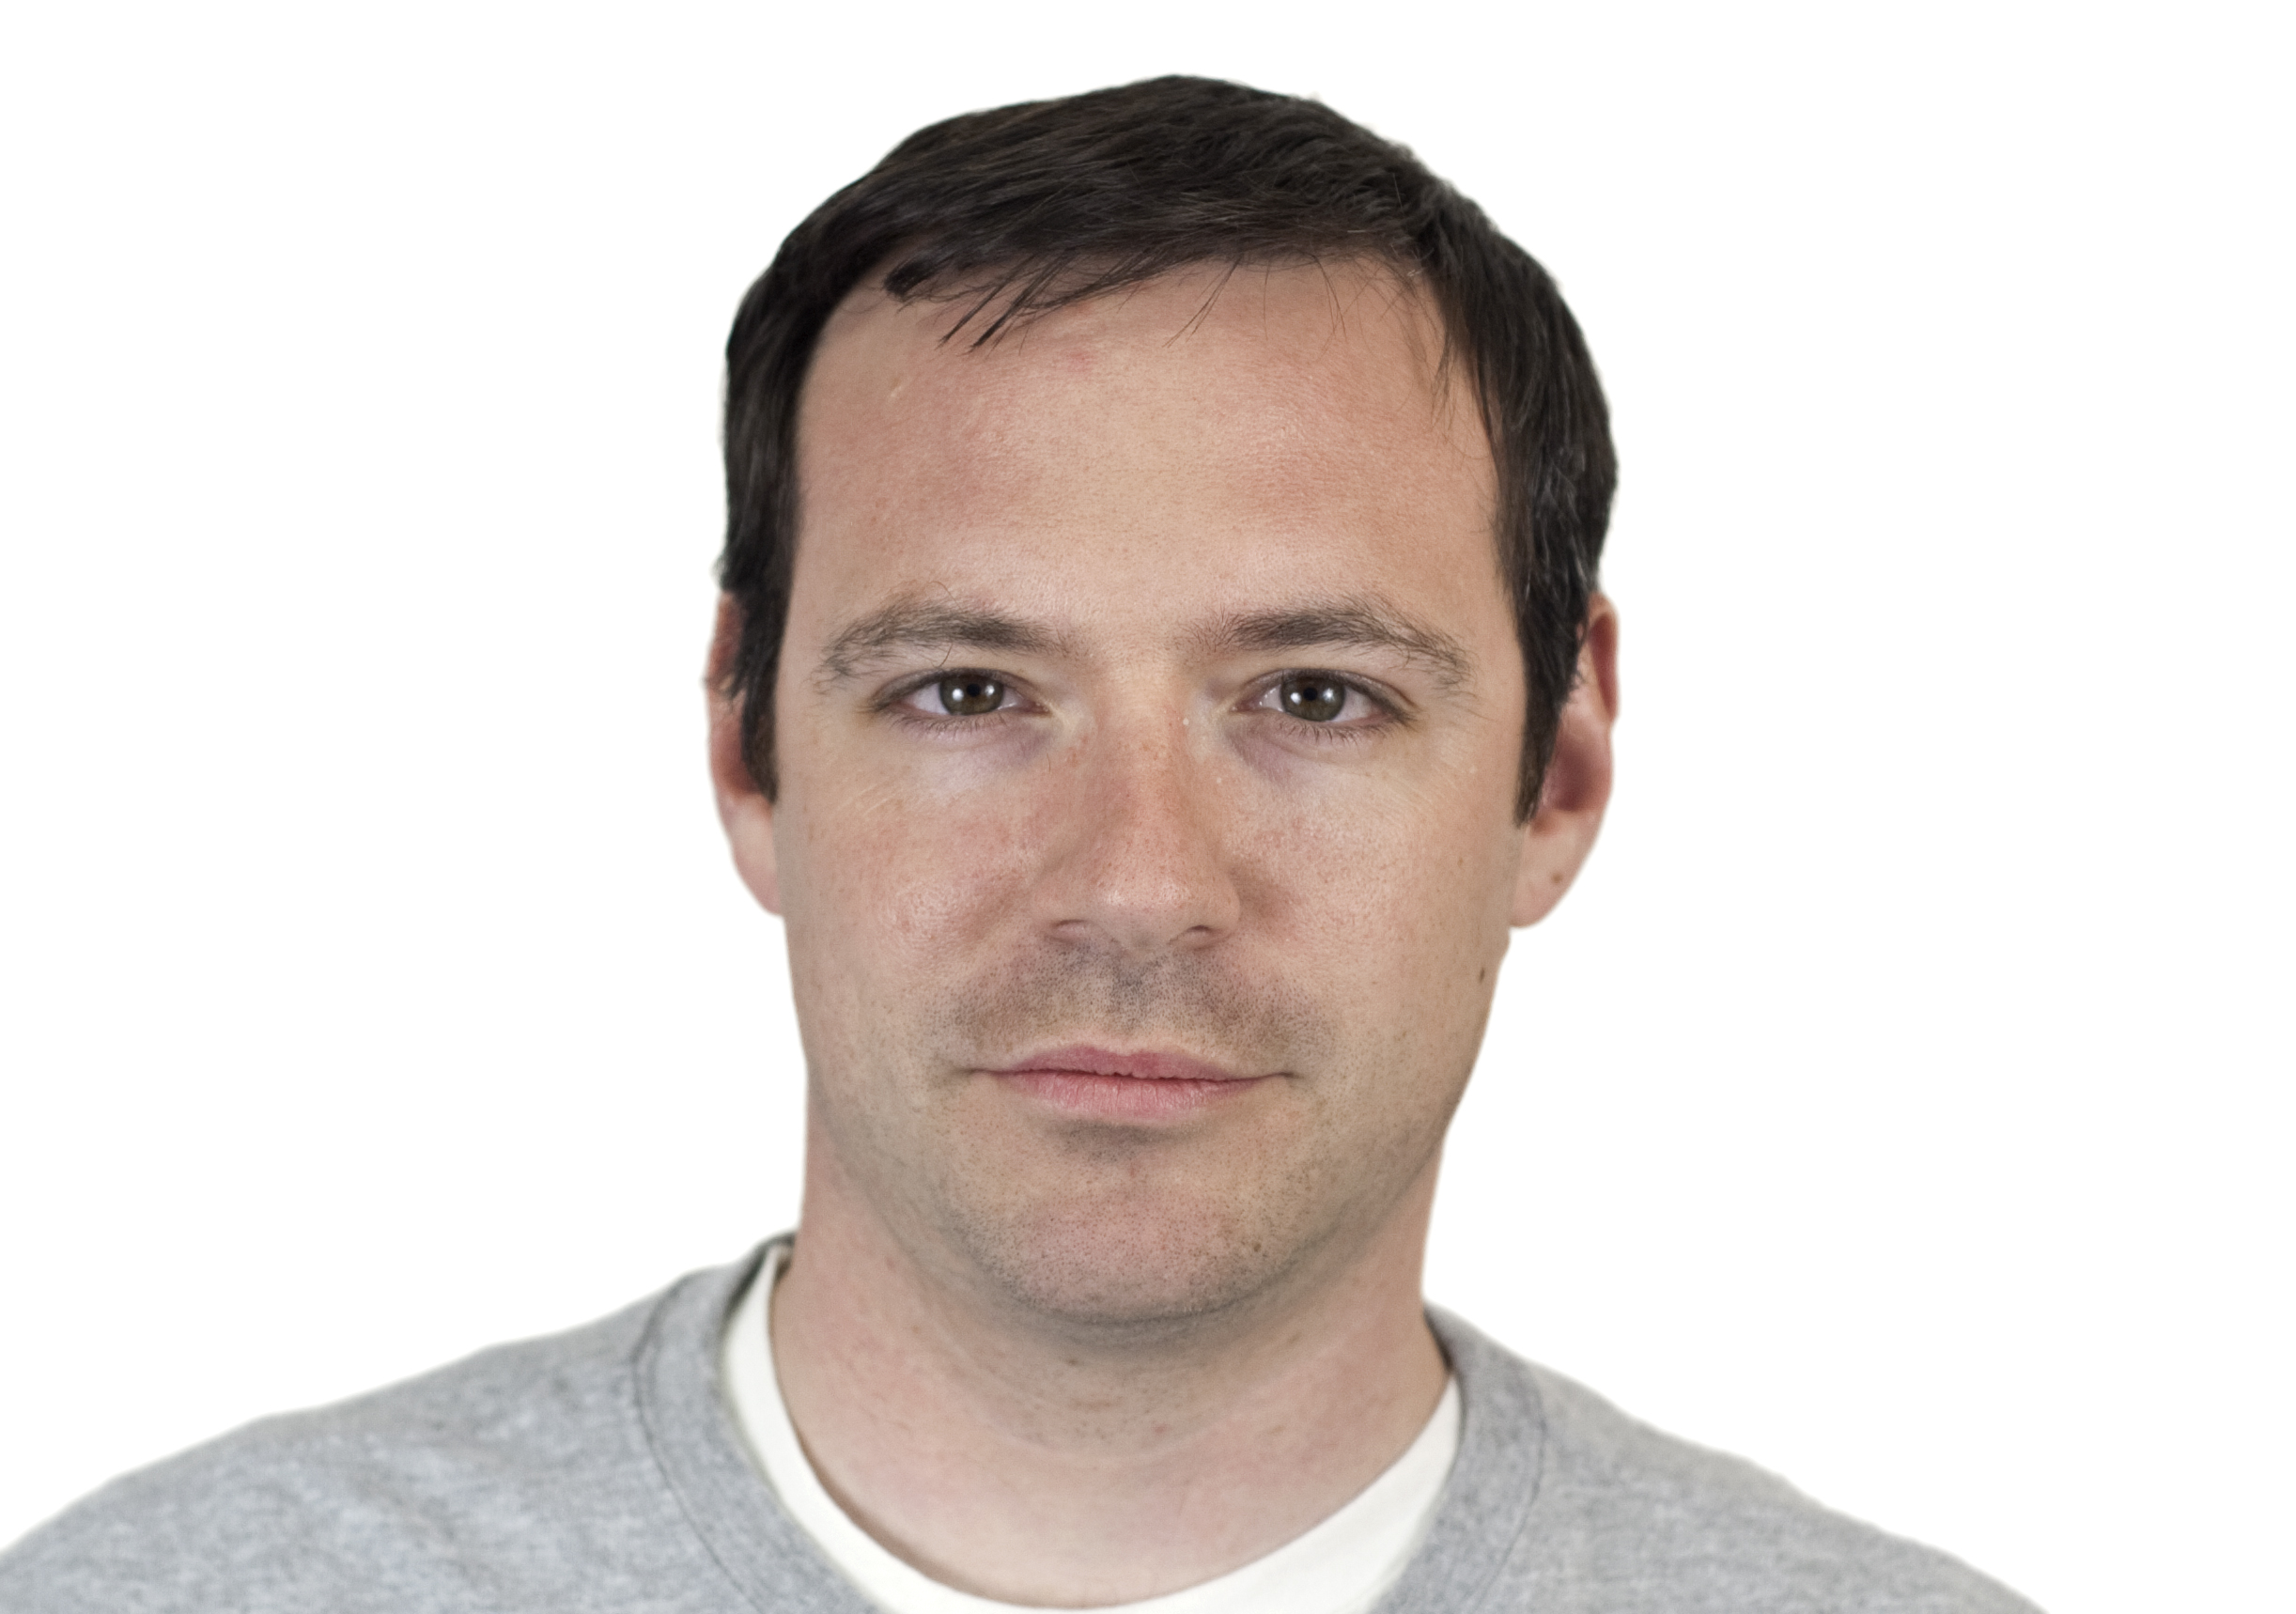
\includegraphics[width=0.26\textwidth]{graphics/study/human.jpg}}
      
\caption{The Entities used in the survey.}
\label{fig:used-entities}

\end{figure}
The focus of the pictures is on the faces of the figures, as this would also be the main focus during a job interview. Furthermore, two of the figures have atypical features. Figure \ref{fig:image-2} depicts a human face with the rest of the body being entirely mechanical, whereas Figure \ref{fig:image-4} depicts a human head with a portion of the skull missing, indicating that it is a robot.

\section{Participants}
A total of thirty people were recruited for the survey. Fifteen were men, 12 were women, and three identified as non-binary. The age of the participants ranged from 17 to 65 years. The majority of the participants were under the age of 30, with only three over the age of 30 (ages 55 and 65), resulting in a mean age of 26.5. With a total of 27, almost all participants were from Europe, with only three from America.

\section{Method}
This research aims to assess the appearance of various robot recruiters to draw conclusions about their acceptability and determine whether they fall into the uncanny valley. To do this, the participants completed a web-based questionnaire in which they had to rate eight images of possible robot recruiters with varying human-likeness and one image of a real human, as seen in Figure 6.1. Before evaluating the robot recruiters, the participants were required to read a brief introductory paragraph. In this text, the following task was described, and the participants were instructed to envision themselves at a job interview employing robot recruiting. Therefore, this introduction should place the chosen entities in the proper context for the rating task. \\
The participants had to rate each of the nine photographs individually in the evaluation assignment. For each picture four 7-point scales between polar adjectives: mechanical/human-like, artificial/lifelike, strange/familiar and not eerie/very eerie were given. In addition, the participants had to indicate how much they liked the picture of the robot recruiter with a simple liking question. Figure \ref{fig:evaluation_task} depicts the exact appearance of the evaluation task questions. The used expressions were also translated into German for better comprehension because most participants were German speakers.
\begin{wrapfigure}[]{r}{0.65\textwidth} %this figure will be at the right
    \centering
    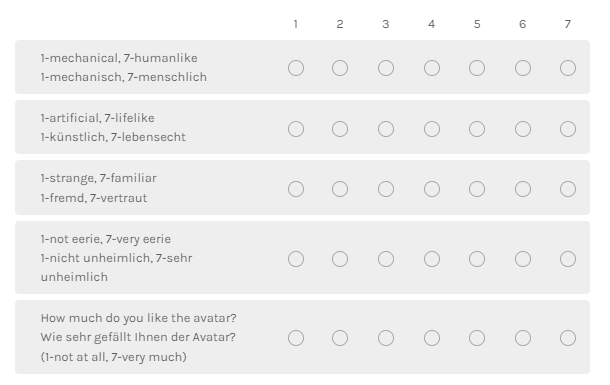
\includegraphics[width=0.65\textwidth]{graphics/evaluation_task.png}
    \caption{Questions used in the evaluation task.}
    \label{fig:evaluation_task}
\end{wrapfigure}
The first two scales (mechanical/human-like, artificial/lifelike)  have the task of inquiring about the perceived human likeness of the figure for the participant. The other two scales (strange/familiar, not eerie/very eerie) are responsible for evaluating the participants' liking or disliking of the figures. This thesis has opted to use the still commonly used term "familiar" to describe the sympathy toward the robot recruiters. To give the term "familiar" a greater significance a simple liking question (How much do you like the avatar?) was added to each assessment task of the robot recruiter. This serves to gather more evidence of the connection between familiarity toward a entity and liking an entity.\\
Before beginning the evaluation task, the participants were asked to rate how much they notice the usage of computer graphics in new films and whether they think this is a positive or negative development. Since films often use computer-generated characters with varying degrees of human-likeness, this question was designed to assess participants' prior experience with virtual characters and the possible prior recognition of the uncanny valley.


\section{Results}

\begin{wrapfigure}[]{r}{0.7\textwidth} %this figure will be at the right
    \centering
    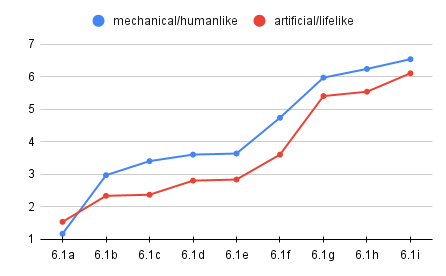
\includegraphics[width=0.7\textwidth]{graphics/result/result1.png}
    \caption{}
    \label{fig:result1}
\end{wrapfigure}

\begin{wrapfigure}[]{r}{0.7\textwidth} %this figure will be at the right
    \centering
    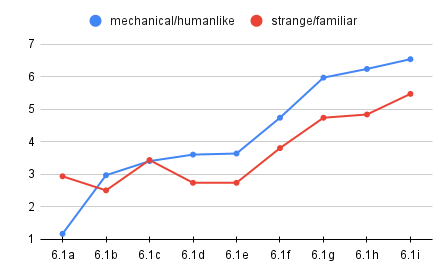
\includegraphics[width=0.7\textwidth]{graphics/result/result3.png}
    \caption{}
    \label{fig:result3}
\end{wrapfigure}

\begin{wrapfigure}[]{r}{0.7\textwidth} %this figure will be at the right
    \centering
    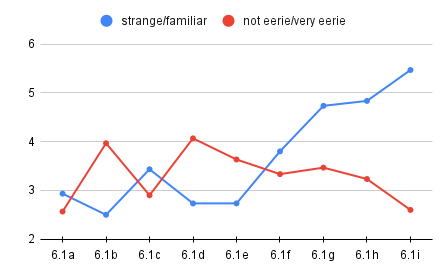
\includegraphics[width=0.7\textwidth]{graphics/result/result2.png}
    \caption{}
    \label{fig:result2}
\end{wrapfigure}

\begin{wrapfigure}[]{r}{0.7\textwidth} %this figure will be at the right
    \centering
    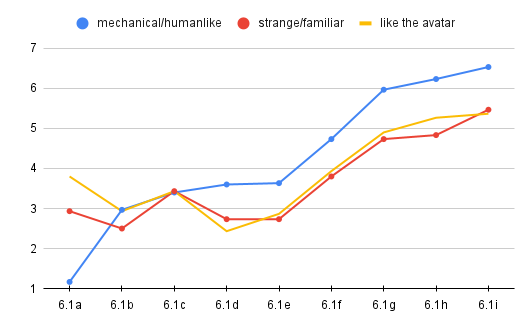
\includegraphics[width=0.7\textwidth]{graphics/result/result4.png}
    \caption{}
    \label{fig:result4}
\end{wrapfigure}


\section{Discussion}

%TODO Ehmer cite doppelt